% -*- TeX-master: "master.tex" -*-
\section{Relativity}
Consider two \emph{inertial} frames $S$ and $S'$ with coordinates denoted as $(t,x,y,z)$ and $(t',x',y',z')$ respectively, and coordinated aligned. If $S'$ moves relative to $S$ in the $+x$ direction, with velocity $v$, the coordinates are related in Newtonian mechanics by a Galilean Transformation:
\begin{definition}[Galilean Relativity]
  Galilean Relativity is defined by the transformation from $S$ to a moving frame $S'$. The key assumption is that \emph{time} is the same in every reference frame:
  \begin{align*}
    t=t'
  \end{align*}
  So if $S'$ is moving relative to $S$ in the $+x$ direction with velocity $v$, we have:
  \begin{align*}
    t'=t\quad x'=x-vt\quad y'=y\quad z'=z
  \end{align*}
  Which is called a \emph{Galilean Transformation}
\end{definition}

\emph{Special Relativity} instead assumes the \underline{speed of light} $c$ is the same in every reference frame.

In order to measure the speed of light, it has to travel over some distance in some time, $\therefore$ define an event:
\begin{definition}[Event]
  An event is defined by a physical occurance (light emission for example). It can be defined to occur at the origin of $S$ and $S'$, A second event at $(t,x,y,z)$ or $(t',x',y',z')$ occurs at a position denoted by the coordinates used in a given inertial frame, $S$ or $S'$
\end{definition}

Spacetime then is the collection of our events, the set of which forms a geometry.

Our assumption that $c(t,x,y,z)=c(t',x',y',z')$ implies that, if we use our two events above:
\begin{gather*}
  c=\frac{\sqrt{x^2+y^2+z^2}}{t}=\frac{\sqrt{(x')^2+(y')^2+(z')^2}}{t'}
\end{gather*}
We can then get a quantity that should be equal in all reference frames:
\begin{align*}
  c^2t^2-(x^2+y^2+z^2)=c^2(t')^2-((x')^2+(y')^2+(z')^2)=0
\end{align*}
We can use this quantity to define a sense of distance in spacetime:
\begin{definition}[Spacetime Separation]
  The distance in spacetime from the origin is defined by $\Delta s$:
  \begin{gather*}
    (\Delta s)^2\equiv c^2t^2-(x^2+y^2+z^2)
  \end{gather*}
  An equivalent assumption for special relativity is that the spacetime distance $\Delta s$ is the same in all inertial frames, i.e.\ it is invariant; invariants are \emph{very} useful quantities.
\end{definition}

\subsection{Light Cone}
Earlier we showed that $\Delta s$ for light is $0$. For a general particle, its velocity is always less than $c$, so in the equation for $\Delta s$, the $t$ term dominates, giving $(\Delta s)^2>0$. Note that if $(\Delta s)^2<0$, even light cannot get there. We then define the three regimes of separation:
\begin{table}[H]
  \centering
  \begin{tabular}{ccc}
    $(\Delta s)^2$ & Name & Note \\\hline
    $>0$ & Time-like & Ordinary Masses \\
    $=0$ & Light-like & Particles that travel at $c$ \\
    $<0$ & Space-like & ``Tachyonic'' matter with $v>c$
  \end{tabular}
  \caption{Spacetime Separation Categories}
\end{table}
This then gives the sense that $(\Delta s)^2=0$ forms a surface in 4-space, we call it the light cone:
\begin{figure}[H]
  \centering
  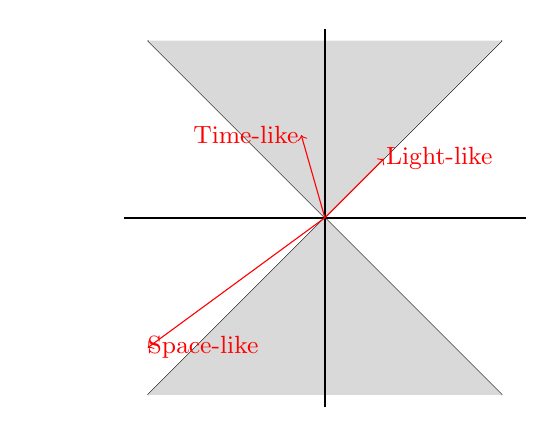
\begin{tikzpicture}[scale=1.5]
    \def\b{0.2} % semi-minor axis
    \pgfmathsetmacro{\h}{(1 + sqrt(1 + 4*\b^2)) / 2}
    \pgfmathsetmacro{\a}{sqrt(\h)}
    \draw (-1.5, -1.5) -- (1.5,  1.5);
    \draw (-1.5,  1.5) -- (1.5, -1.5);
    \fill[gray!30] (0,0) -- (1.5,1.5) -- (-1.5,1.5);
    \fill[gray!30] (0,0) -- (-1.5,-1.5) -- (1.5,-1.5);
    % \draw (0,  \h) ellipse [x radius = \a, y radius = \b];
    % \draw (0, -\h) ellipse [x radius = \a, y radius = \b];
    \draw [thick] (0,-1.6) -- (0,1.6);
    \draw [thick] (-1.7,0) -- (1.7,0);
    \draw [->, red] (0,0) -- (0.5,0.5) node {\hspace{4em}\small Light-like};
    \draw [->, red] (0,0) -- (-0.2,0.7) node {\hspace{-4em}\small Time-like};
    \draw [->, red] (0,0) -- (-1.5,-1.1) node {\hspace{4em}\small Space-like};
  \end{tikzpicture}
  \caption{The Light Cone}
\end{figure}
The gray shaded area is the accessible region of spacetime by light, the lightcone.

\subsection{Time Dilation}
Consider an object in frame $S$ moving with velocity $\vb{v}$, $\vb{s}\vdot\dd{\vb{x}}=\vb{v}\dd{t}$. Choose frame $S'$ to be ``co-moving'' with the object, so that the object is always at rest at the origin.

A small movement from event one to event two is:
\begin{align*}
  (\Delta s)^2&=(c\Delta t')^2\quad \text{in $S'$}\\
  &=(c\Delta t)^2-(\Delta x^2+\Delta y^2+\Delta z^2)\quad \text{in $S$}\\
\end{align*}
As an infinitesimal:
\begin{align*}
  (c\dd{t}')^2&=(c\dd{t})^2-(\dd{x}^2+\dd{y}^2+\dd{z}^2)\\
  &=\qty(c^2-v^2)\dd{t}^2
\end{align*}
So we define $t'$ in the $S'$ frame the proper time $\tau$, such that:
\begin{align*}
  \dd{t}'&\equiv\dd{\tau}=\sqrt{1-\frac{v^2}{c^2}}\equiv\sqrt{1-\beta^2}\\
  \beta&\equiv\frac{v}{c}
\end{align*}
Note that $\dd{\tau}\leq\dd{t}$, so \emph{moving clocks appear to run slow}
\begin{note}
  This is not an idle Observation. A large fraction of cosmic radiation at sea level comes from muons produced in pion decays in the upper atmosphere. THe muon lifetime of $\SI{2.2}{\micro\s}$ would imply that muons travelling at $c$ would only get $\sim\SI{600}{\m}$ if Galilean transformations are correct. Yet $~\frac12$ the muons produced at $\SI{2}{\km}$ make it to sea level (including losses from scattering). This means the muons were travelling at least at $\beta>0.976$ in our frame.
\end{note}

\subsection{Four-Vectors and Minkowski Space}
Express the coordinates for an event $(t,x,y,z)$ as a 4-dimensional vector:
\begin{align*}
  \vb{x}=\bmqty{ct\\x\\y\\z}=\bmqty{ct\\\vb{r}}
\end{align*}
In ordinary space (Euclidean): $\abs{\vb{x}}^2=c^2t^2+x^2+y^2+z^2$ (not what we want).

Define length in Minkowski space:
\begin{align*}
  \abs{\vb{x}}^2=\vb{x}\vdot\vb{x}=
  \vb{x}^T
  \underbrace{\bmqty{\dmat{1,-1,-1,-1}}}_{\text{``metric tensor'' }g}\vb{x}
  =c^2t^2-(x^2+y^2+z^2)
\end{align*}

The 4-dim space with metrix $g$ as above is called ``Minkowski space'',
``Euclidean space'' (flat space) has the identity $\id_{4\times4}$ as a metric. Special relativity says the length of a 4-vector in Minkowski space is the same in all inertial frame, i.e.\ invariant.

We began with the Galilean relationship between frames $S$ and $S'$. The real question is: What is the general form of the transformation between $S$ and $S'$ that conserves length in Minkowski space? \emph{Answer}: Homogeneous \emph{Lorentz Transformation}

Physics does not depend on (our definition of) absolute position or time. (This is a fundamental assumption of relativity).

Shifting the origin of $S$ must simply shift the origin of $S'$: $x\to x+a\implies x'\to x'+a$, so a transformation $L(x+a)=L(x)+a'$. Try $x=0$, $L(a)=L(0)+a'$, so $L(x+a)=L(x)+L(a)-L(0)$, define $L'(x)=L(x)-L(0)$ so that $L'(x+a)=L'(x)+L'(a)$, so $L(x)$ is a linear function of  $x$ plus a fixed offset.

Any linear transformation can be written sa a Poincare transformation $x'=Lx+a$; $L$ is a $4\times4$ matrix, $a$ translates the origin. Since physics is independent of where we place the origin, we only care about ``homogeneous Lorentz transformations'' (HLT) where we drop $a$.

\subsection{What do we know about $L$?}
We know $L$ must conserve 4-vector length\footnote{Note 4-vectors will be non-bolded from here on}:
\begin{align*}
  \abs{x}^2=x^T g x\iff \abs{x'}^2=(x')^T gx'=x^TL^TgLx
\end{align*}
So we need $\boxed{L^T gL=g}$.

If we consider components, $L_{ki}g_{kl}L_{lj}=g_{ij}$ forms 16 real equations, $g$ is symmetric, so there are $10$ constraints $\implies$ $\boxed{L\text{ has 6 d.o.f}}$ What are they?

Recall rotation matrices $A$ were defined by requiring conservation of length of the 3-vector in cartesian space:
\begin{align*}
  \abs{x}^2=\underbrace{c^2t^2}_{\text{untouched}}
  -\underbrace{\qty(x^2+y^2+z^2)}_{\text{conserved by }A}
  =\text{const.}
\end{align*}
So, rotations are a 3-D subset (subgroup) of an HLT.\@ $\therefore$ Euler angles are 3 of the d.o.f., what are the others?

Consider our frames $S$ and $S'$, were the origin of $S'$ is moving at constant velocity with respect to $S$: $x=v_xt,y=v_yt,z=v_zt$. We can always rotate $S$ and $S'$ so that the $x,x'$ are parallel to $\vb{v}$ (After all we just said rotations were a subset of HLT). Hence we can write the transformation as:
\begin{align*}
  \bmqty{ct'\\x'\\y'\\z'}=\bmqty{L_{00}&L_{01}\\L_{10}&L_{11}\\ &&1\\&&&1}
  \bmqty{ct\\x\\y\\z}
\end{align*}
Since $L$ satisfies $L^TgL=g$:
\begin{align*}
  L_{00}^2-L_{10}^2&=1\\
  L_{01}^2-L_{11}^2&=1\\
  L_{00}L_{01}-L_{10}L_{11}&=0
\end{align*}
The origin of $S'$ is $x'=0$, this means $0=L_{10}ct+L_{11}x$, which must satisfy $x=vt$, so $\beta\equiv\frac{v}{c}=-\frac{L_{10}}{L_{11}}$. Working out other combinations means:
\begin{align*}
  \bmqty{L_{00}&L_{01}\\L_{10}&L_{11}}=
  \bmqty{(\pm)\gamma&(\mp)\gamma\beta\\(\mp)\gamma\beta&(\pm)\gamma}
\end{align*}
Where the signs are arbitrary, and the lorentz factor $\gamma$ is:
\begin{align*}
  \gamma\equiv\frac1{\sqrt{1-\beta^2}}
\end{align*}
At low velocity ($\beta\to0$), we must recover the identity $L\to\smqty[\pm1\\&\pm1]$, so we choose the plus branch, hence we have:
\begin{align*}
  \boxed{L=\bmqty{\gamma&-\gamma\beta\\-\gamma\beta&\gamma\\&&1\\&&&1}}
\end{align*}
This is called a \emph{Lorentz boost along $x$}.

\begin{remark}
  Other solutions with different choices of $+$ and $-$ signs, such as:
  \begin{align*}
    L_{1}=\bmqty{\gamma&-\gamma\beta\\\gamma\beta&-\gamma}
    \quad\text{or}\quad
    L_{2}=\bmqty{-\gamma&\gamma\beta\\-\gamma\beta&\gamma}
  \end{align*}
  Represent reflections of the axes, $L_1$ represents a flip along the $x$ axis, or space inversion, and $L_2$ represents a flip along the $t$ axis, time reversal.

  These possibilities are not a part of \underline{continuous} Lorentz transformations, but could be interesting operators for other purposes.
\end{remark}

\subsection{General Boosts}
When the velocity between $S,S'$ is not along 1 axis, we can generalize with $\vb{r}_\|$ and $\vb{r}_\perp$, the parallel and perpendicular positions relative to the frame velocity $\vb{v}$, they are given by:
\begin{align*}
  \vb{r}_\|=\frac{(\vb{r}\vdot\bm{\beta})}{\beta^2}\bm{\beta}
  \qquad
  \vb{r}_\perp=\vb{r}-\vb{r}_\|
\end{align*}
So we have the following relationship between primed and unprimed variables:
\begin{align*}
  ct'&=\gamma ct-\gamma\beta\abs{\vb{r}_\|}=
  \gamma ct-\gamma(\vb{\bm{\beta}\vdot\vb{r}})\\
  \vb{r}'&=-\gamma\bm{\beta}ct+\gamma\vb{r}_\|+\bm{r}_\perp
  =-\gamma\bm{\beta}ct+\vb{r}+
  \frac{\gamma-1}{\beta^2}(\vb{r}\vdot\bm{\beta})\bm{\beta}  
\end{align*}
For a general $\beta$ we have:
\begin{align*}
  L_B=\bmqty{\gamma&-\gamma\bm{\beta}^T\\-\gamma\bm{\beta}
    &\id+(\gamma-1)\bm{\beta\beta}^T/\beta^2}
\end{align*}
In block matrix notation. Note that since $\beta$ has 3 components, these are our misisng 3 degrees of freedom.

A homogeneous Lorentz transform is a Boost and a rotation: $L_B L_A\equiv L$. A Poincare transform: $\vb{x}'\to L_BL_A\vb{x}+\vb{a}$, where $\vb{a}$ shifts origin.
\begin{note}
  We have the following properties of $L_B$ for boosts:
  \begin{enumerate}
  \item When $\beta\to0$, $L\to\id$
  \item $L_B^{-1}$ is formed by taking $\bm{\beta}\to-\bm{\beta}$
  \item $L_B$ is symmetric; $L_A=\smqty[\dmat{1,A}]$, $A$ antisymmetric; $L=L_BL_A$ is mixed.
  \end{enumerate}
\end{note}
\subsubsection{Addition of Velocities}
If $\bm{\beta}\|\bm{\beta}'$, define motion to be $x$-direction, we have:
\begin{align*}
  L'_BL_B=\bmqty{\gamma'&-\gamma'\beta'\\-\gamma'\beta'&\gamma'}
  \bmqty{\gamma&-\gamma\beta\\-\gamma\beta&\gamma}=
  \bmqty{\gamma'\gamma(1+\beta'\beta)&-\gamma'\gamma(\beta+\beta')\\
    -\gamma'\gamma(\beta+\beta')&\gamma'\gamma(1+\beta'\beta)}
\end{align*}
This is equivalent to \underline{one} transform $L_B''$ with:
\begin{align*}
  \beta''=\frac{\beta+\beta'}{1+\beta'\beta}
\end{align*}
With $\beta''<1$ still.

\textbf{Warning}: In general $L'_BL_B\neq L_BL'_B$, matrix is \underline{not} symmetric, so two proper Lorentz transforms (PLT) do \underline{not} add up to a PLT. \underline{But} two HLT \underline{do} add ip to a HLT (Call them $\Lambda$), in particulat, $L'_BL_B=L_B''L_A$, two PLTS add to a single PLT and a rotation.

\subsubsection{Lorentz Group}
The Lorentz group, $SO(3,1)$ HLT are orthogonal $4\times4$ matrices $O(4)$ with determinant $\det\Lambda=+1$, which means they are special $SO(4)$, and with the metric $\mathrm{diag}(1,-1,-1,-1)$, this is called $SO(3,1)$
\begin{note}[Group Structure of HLT]
  \begin{enumerate}
  \item Identity exists, $I=\id$
  \item Inverse exists, since $\Lambda^T\Lambda=\id$, $\Lambda^{-1}=\Lambda^T$
  \item Associative:
    \begin{align*}
      \Lambda_i(\Lambda_j\Lambda_k)=(\Lambda_i\Lambda_j)\Lambda_k
    \end{align*}
    This is always true for matrices.
  \item Closure: $\Lambda_1\Lambda_2=\Lambda_3$, subproof:
    \begin{align*}
      (\Lambda_1\Lambda_2)^T(\Lambda_1\Lambda_2)=
      \Lambda_2^T\Lambda_1^T\Lambda_1\Lambda_2=\id
    \end{align*}
    Hence $\Lambda_3$ is also HLT.
  \end{enumerate}
\end{note}
\begin{TODO}
  Demonstration that two PLTs do not give a PLT
\end{TODO}
\subsection{Notation}
We note a 4-vector with greek indices, such as $x^\mu$, with $\mu=0,1,2,3$, the upper index means it is a contravariant vector, with indices:
\begin{align*}
  x^\mu=(ct,x^i)
\end{align*}
Where a roman index, such as $i$ denotes a 3-vector, with $i=1,2,3$

Under a Lorentz transform: $x^{\prime\mu}=\Lambda^\mu_\nu x^\nu$. We sum matched upper/lower greek indices (Einstein convention). The elements of $x^{\prime\mu}$ are:
\begin{align*}
  x^{\prime\mu}=(\gamma(x^0-\beta x^1),\gamma(x^1-\beta x^0),x^2,x^3)
\end{align*}
With the transform as before. Where did the lower index come from? The 1-Form (meaning 1 index) $x_\mu$ (lower Greek index) comes from $x^Tg$ ``covariant'' such that:
\begin{align*}
  x_\mu=(ct,-x^i)\equiv (ct,x_i)
\end{align*}
We ``lowered'' the index on $x$ by multiplying with the metric. What is the metric?
\begin{align*}
  g_{\mu\nu}=\vu{e}_\mu\vdot\vu{e}_\nu
\end{align*}
Given some basis, the vectors: $u$ and $v$, the product $u\vdot v=u^\mu\vu{e}_\mu\vdot v^\nu\vu{e}_\nu$

\begin{definition}[The Metric]
  The metric is a \emph{tensor} of rank 2 that contains the lengths and angles between basis vectors.
  \begin{itemize}
  \item In \emph{Minkowski} space, $g_{\mu\nu}$ is diagonal, but it is not a requirement.

    There is a corresponding tensor that ``raises'' indices, called the inverse metric $g^{\mu\nu}$
  \item In \emph{Minkowski} space, $g^{\mu\nu}$ has the same matrix form as $g_{\mu\nu}$, generally, $g^{\alpha\beta}g_{\beta\gamma}=\delta^{\alpha}_\gamma$
  \item The trace $g^{\alpha\alpha}=\delta^\gamma_\alpha\delta^\alpha_\gamma=4$ in 4 dimensions
  \end{itemize}
\end{definition}
We can formally move between upper and lower indices:
\begin{align*}
  x^\mu=g^{\mu\nu}x_\nu\qquad x_\mu=g_{\mu\nu}x^\nu
\end{align*}
\begin{note}
  Tensor notation, tensors are defined as having at least two indices, and are combinations of vectors via a tensor product:
  \begin{gather*}
    T^{\alpha\beta}=u^\alpha v^\beta\iff \bm{T}=u\otimes v\\
    T^{\alpha\beta\gamma}=u^\alpha v^\beta w^\gamma\iff \bm{T}=u\otimes v\otimes w
  \end{gather*}
  Where $\bm{T}$ is the tensor object.

  You can still freely move between upper and lower indices
  \begin{gather*}
    T_{\alpha\beta}=g_{\mu\alpha}g_{\nu\beta}T^{\mu\nu}\\
    T_\alpha^\beta=g_{\alpha\mu}T^{\mu\beta}
  \end{gather*}
  You just need a metric for each index you want to raise/lower
\end{note}
We can then see how each of the various objects transform under Lorentz transformations

\begin{itemize}
\item 1-form (vector) $x'_\mu=\Lambda^\mu_\nu x^\nu$
\item Tensor $T^{\prime\beta}_\alpha = \Lambda_\alpha^\gamma \Lambda_\delta^\beta T_\gamma^\delta$
\item Scalar $a'\vdot b'=\Lambda^\mu_\nu a^\nu\Lambda_\nu^\sigma b_\sigma=a^\nu b_\nu=a\vdot b$ which is invariant
  \begin{note}[Dot Product]
    Due to the metric of Minkowski space, the 4 vector dot product is:
    \begin{align*}
      a\vdot b\equiv a_\mu b^\mu=a^\mu b_\mu=a^0b^0-\vb{a\vdot b}
    \end{align*}
  \end{note}
\end{itemize}
We should now move onto a few physical quantities.

Imagine following the trajectory of a particle through 4-space. The trajectory will be $x^\mu(\lambda)$, where $\lambda$ is a parameter that monotonically varies along the curve. At any point $\lambda_0$ we may define a tangent 4-vector:
\begin{align*}
  \eta^\mu=\eval{\dv{x^\mu}{\lambda}}_{\lambda_0}
\end{align*}
For time-like particles, it is convenient to choose $\lambda=\tau$, the proper time:

\textbf{Proper Velocity}: $\bm{\eta}=\pdv{\vb{x}}{\tau}$ and thus the 4-velocity is: $\eta^\mu=\dv{x^\mu}{\tau}$.

If $S'$ is at rest with respect to a particle and moves with velocity $\vb{v}$ with respect to $S$, we have:
\begin{align*}
  x^\mu &= (ct,x^i) = (\gamma c\tau, \gamma v^i\tau)\\
  \eta^\mu &= (\gamma c, \gamma v^i)
\end{align*}
Notice that $\eta^2=\eta\vdot\eta=\gamma^2(c^2-v^2)=c^2$

Much more useful is the 4-momentum:
\begin{align*}
  p^\mu&=m\eta^\mu=(\gamma mc, \gamma mv^i)
\end{align*}
\begin{note}
  The components of the 4-momentum are useful to note, as the 3-vector components are just a boosted 3-momentum:
  \begin{align*}
    \vb{p}=m\gamma \vb{v}
  \end{align*}
  And the time component is related to the energy:
  \begin{align*}
    p^0=\frac{E}{c}=\gamma m c
  \end{align*}
\end{note}
The square of the 4-momentum is also useful:
\begin{align*}
  p^2=m^2c^2 = \qty(E/c)^2-(\vb{p\vdot p})
\end{align*}

\subsection{Conventions and ``Gotchas''}
\begin{enumerate}
\item In particle physics it is traditional to work in ``units of c''. The consstant speed of light is dimensionful and sets the natural scale of calculations. This means it is appropriate to define $\boxed{c=1}$. When units are required, we go back and put in however many $c$'s are required. Thus we have:

  $x^\mu\to(\tau,x^i)$ with $\tau$ in meters

  $p^\mu\to(E,\vb{p})$ with $E,m,\abs{\vb{p}}$ all in units of energy (eV)
\item \textbf{Metrics}: We have chosen $g_{\mu\nu}=\mathrm{diag}(1,-1,-1,-1)$, this is sensible as $p^2=E^2-\abs{\vb{p}}^2=m^2>0$
  \begin{enumerate}[label=\alph*)]
  \item Another choice often used in astrophysics is $g_{\mu\nu}=\mathrm{diag}(-1,1,1,1)$, then at $t=0$, $x^2=\abs{\vb{x}}^2$ However $p^2=-m^2<0$ which is technically valid but can be confusing.
  \item Also, sometimes (particularly in classical field theory), you need to stick with a Euclidean metric $\eta_{\mu\nu}=\mathrm{diag}(1,1,1,1)$, then some coordinates become \underline{complex}: $x^I=(ict,x^i)$
  \end{enumerate}
\item \textbf{Indices}: Some computer programs (you likely use) unfortunately chose to write 4-vectors as $x^{\tilde{\mu}}=(\vb{x},ct)$, with $\tilde{\mu}=1...4$. This was never necessary, and has led to many errors over the years.
\end{enumerate}
You have been warned.

\subsection{Relativistic Kinematics}
When we examine kinematics in the Newtonian ``classical'' limit, we invoke conservation laws. Consider a collision $A+B\to C+D$:
\begin{enumerate}
\item \underline{Mass} is conserved: $m_A+m_B=m_C+m_D$
\item \underline{Momentum} is conserved: $\vb{p}_A+\vb{p}_B=\vb{p}_C+\vb{p}_D$
\item \underline{Kinetic Energy}
  \begin{enumerate}[label=\alpha*)]
  \item decreases if collision is sticky $T_A+T_B>T_C+T_D$
  \item increases if collision is explosive $T_A+T_B<T_C+T_D$
  \item conserved if elastic $T_A+T_B=T_C+T_D$
  \end{enumerate}
\end{enumerate}

In relativistic kinematics, we assume all interactions are \emph{local}. (We will see why later -- it is in fact a very strong statement about the nature of the Universe, but it is also necessary for consistency.)

\begin{figure}[H]
  \centering
  \begin{tikzpicture}
    TODO
  \end{tikzpicture}
  \caption{Collision Picture}
\end{figure}

Our picture of collisions is 2 particles under free motion enter a ``black box'' in which they exchange a force, and then they travel off freely again.

\begin{enumerate}
\item \underline{Total Energy} is conserved
\item \underline{Momentum} is conserved
  \begin{enumerate}
  \item These are combined to give conservation of 4-momentum:
    \begin{align*}
      p^\mu_A+p^\mu_B=p^\mu_C+p^\mu_D
      \begin{cases}
        E_A+E_B=E_C+E_D\\
        \vb{p}_A+\vb{p}_B=\vb{p}_C+\vb{p}_D
      \end{cases}
    \end{align*}
  \end{enumerate}
\item \underline{Kinetic Energy}
    \begin{enumerate}[label=\alph*)]
  \item decreases if collision is sticky, \underline{mass} increases (particle creation)
  \item increases if collision is explosive, \underline{mass} decreases (particle decay, eg)
  \item conserved if elastic, so is mass
  \end{enumerate}
\end{enumerate}
We have given up conservation of mass, for conservation of energy

\begin{example}
  Two lumps of clay, each with mass $m$, collide head-on with speeds $\frac35c$. What is the final mass $M$ of the lump?
  \begin{align*}
    E_1+E_2&=E_M\\
    \vb{p}_1+\vb{p}_2&=\vb{p}_m=0
  \end{align*}
  Note we make a good choice of reference frame such that we end up in the rest frame of the final mass $M$, and the two lumps collide head on. Since $c=1$, we simply have $M=2E_m$, with $E_m$ given by:
  \begin{align*}
    E_m=\gamma m=\frac{m}{\sqrt{1-(3/5)^2}}=\frac54m
  \end{align*}
  Hence:
  \begin{align*}
    \boxed{M=\frac52m}
  \end{align*}
\end{example}
\begin{example}
  A particle of mass $M$ at rest decays into two particles of mass $m$. What is the \emph{speed} of each piece as it flies away?

  Speed is not a natural quantity (like $E$ or $p$), so we should find one of those and use:
  \begin{align*}
    \beta=\frac{\abs{\vb{p}}}{E}
  \end{align*}
  To derive the speed.

  So far we only have:
  \begin{align*}
    p^\mu&=p_1^\mu+p_2^\mu\\
    p^2&=M^2\\
    p_1^2=p_2^2=m^2
  \end{align*}
  To go further we should use \emph{invariants}
  \begin{enumerate}[label=\alph*)]
  \item Use $p^2=(p_1+p_2)^2$ and a convenient choice of reference frame such that:
    \begin{align*}
      p&=(M,0,0,0)\\
      p_{1/2}&=(E,0,0,\pm p_z)
    \end{align*}
    We can then expand the square of the sum:
    \begin{align*}
      p^2&=M^2\\
      (p_1+p_2)^2=m^2+m^2+2p_1\vdot p_2
    \end{align*}
    From our choice of frame, we can say:
    \begin{align*}
      p_1\vdot p_2&=E^2+\abs{\vb{p}}^2=2E^2-m^2\\
      \implies M^2&=2m^2+4E^2-2m^2=4E^2
    \end{align*}
    Thus we get:
    \begin{align*}
      E=\frac12M
    \end{align*}
    And for $\abs{\vb{p}}$:
    \begin{align*}
      \abs{\vb{p}}^2=E^2-m^2=\frac14M^2-m^2
    \end{align*}
    So the speed is:
    \begin{align*}
      \boxed{\beta=\sqrt{1-\frac{4m^2}{M^2}}}
    \end{align*}
  \end{enumerate}
\end{example}

\begin{example}
  A pion (135 MeV) decays to two photons. what are $E,\abs{\vb{p}},\beta$ of the photons?

  Using example 2.2:
  \begin{align*}
    E_\gamma&=\frac12M_\pi=67.5\text{MeV}\\
    \abs{\vb{p}_\gamma}^2&=E^2-\cancel{m^2}^0\\
    \implies\beta&=\frac{\vb{p}}{E}=\frac{E_\gamma}{E_\gamma}=1
  \end{align*}
  Good! It should travel at the speed of light

  So a \underline{massless} particle (like a photon), has a 4-momentum:
  \begin{align*}
    p^\mu=E(1,\vu{p})
  \end{align*}

  A \underline{massive} particle can also its 4-momentum written as:
  \begin{align*}
    p^\mu=E(1,\bm{\beta})
  \end{align*}
\end{example}

\begin{example}
  The Bevatron created antiprotons by hitting a fixed target (protons) with a beam of protons. The reaction is $p+p\to p+p+p+\bar{p}$. What was the threshold energy ($E_p^{\text{LAB}}$)

  The lab frame consists of a proton of energy $E$ hitting a stationary proton, and everything in the final state moves.

It is generally easier to work in the \underline{center of momentum} frame (where $\sum p^i=0$ or $\sum\vb{p}=0$), do not be sloppy in nomenclature, this is not center of mass.

In this frame, two particles collide head on and the 4 products are left at rest (at threshold). Using invariants:
\begin{align*}
  \underbrace{(p_1+p_2)^2}_{\text{frame inv.}}
  =(p_3+p_4+p_5+p_6)^2=16m^2
\end{align*}
The quantity above is frame invariant, so it is the same as in the lab frame:
\begin{align*}
  (p_1+p_2)^2_{\text{LAB}}=2m^2+2Em
\end{align*}
So equating these we have:
\begin{align*}
  16m^2=2m^2+2Em\implies E=7m
\end{align*}
This is the power of invariants!
\end{example}
\subsubsection{General Strategy}
\begin{enumerate}
\item Unless the solution is trivial, rewrite in terms of Lorentz scalars (invariants). Try to choose easy ones to evaluate.
\item Evaluate the scalars in \emph{any} frame --- the more straight forward the better.
\item If you need a particular quantity, e.g. $\beta$ of a certain particle, consider regrouping momenta before squaring
\end{enumerate}

\subsection{Mandelstam Invariants}
For the general process $A+B\to C+D$, the following quantities are named:
\begin{align*}
  s\equiv(p_A+p_B)^2&=(p_C+p_D)^2\\
  t\equiv(p_A-p_C)^2&=(p_D-p_B)^2\\
  u\equiv(p_A-p_D)^2&=(p_C-p_B)^2
\end{align*}
If we sum them we get a fairly useful quantity:
\begin{align*}
  s+t+u=m_A^2+m_B^2+m_C^2+m_D^2
\end{align*}
Returning to $pp\to ppp\bar{p}$, we used the invariant $s$ to calculate everything
